\documentclass[11pt]{beamer}
\usetheme{Madrid}
\usepackage[utf8]{inputenc}

\usepackage{hyperref}
\usepackage{amsmath}
\usepackage{amsfonts}
\usepackage{amssymb}
\usepackage{graphicx}
\DeclareMathOperator{\argmin}{argmin}
\usepackage{algorithmic}
\usepackage{algorithm}
\usepackage{wrapfig}
\usepackage{subcaption}
\graphicspath{{.}}

\author{Hongda Li}
\title{A Discussion on The Nesterov Momentum and Variants of FISTA with TV Minmizations Application}
% Informe o seu email de contato no comando a seguir
% Por exemplo, alcebiades.col@ufes.br
\newcommand{\email}{lalala@lala.la}
\setbeamercovered{transparent}
\setbeamertemplate{navigation symbols}{}
%\logo{}
\institute[]{UBC Okangan}
\date{\today}
\subject{Subject Title }

% ---------------------------------------------------------
% Selecione um estilo de referência
\bibliographystyle{IEEEtran}

%\bibliographystyle{abbrv}
%\setbeamertemplate{bibliography item}{\insertbiblabel}
% ---------------------------------------------------------

% ---------------------------------------------------------
\newtheorem{remark}{Remark}
\newtheorem{assumption}{Assumption}

\begin{document}

\begin{frame}
    \titlepage
\end{frame}

\begin{frame}{ToC}
    \tableofcontents
\end{frame}

\section{Introduction}
    \begin{frame}{Paper Under Review}
        \begin{center}
            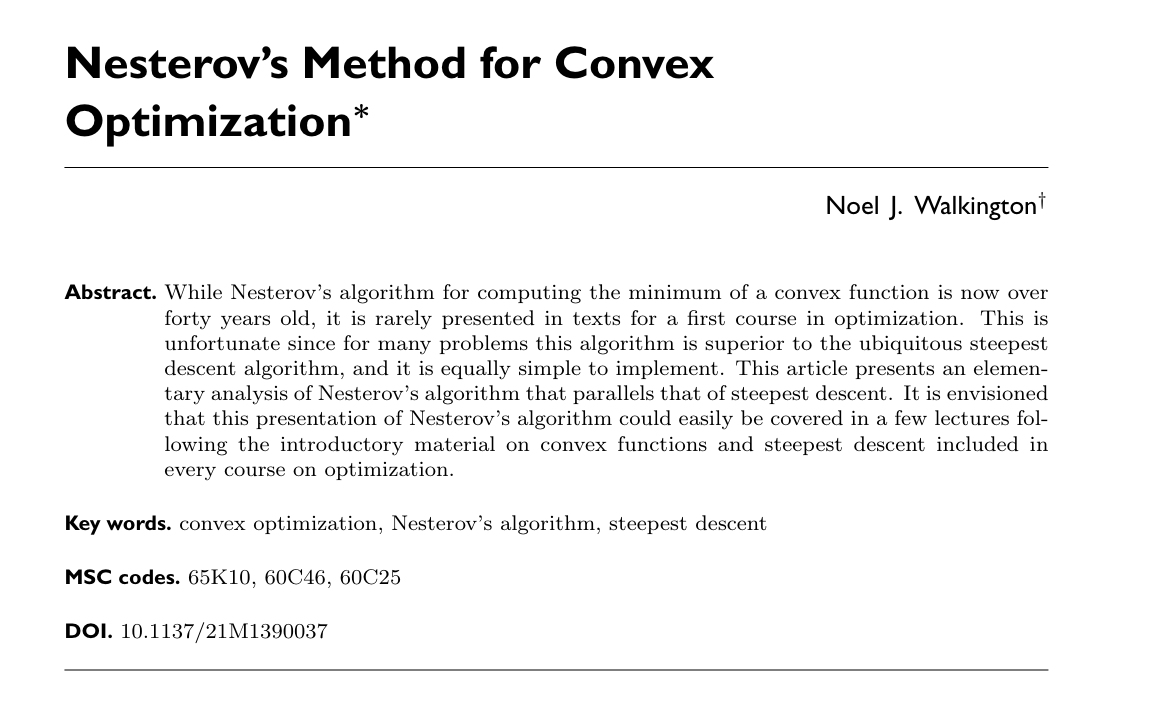
\includegraphics[width=10cm]{Assets/paper-titlepage.png}    
        \end{center}
        Noel J. Walkington, SIAM REVIEW Jun 2023 Education, Volume 65 Number 2, pp. 539-562. \cite{noel_nesterovs_nodate}
    \end{frame}
    \begin{frame}{Presentation Outline and Objective}
        \begin{itemize}
            \item [1.] Introducing the Application of TV Minimization for Signal Recovery.
            \item [2.] Literature Review. 
            \item [3.] Nesterov lower bound complexity claim clarified. 
            \item [4.] Our proof for V-FISTA convergence under strong convexity inspired by \cite[10.7.7]{beck_first-order_nodate}
            \item [5.] Some exciting numerical results for our method, which we refer to as ``The method of Spectral Momentum''. 
        \end{itemize}
    \end{frame}

\section{TV Minimizations}
    \begin{frame}{Total Variance Minimization Formulation}
        Total Variance Minimization (TV) problem recovers the digital signal from observations of a signal with noise. 
        Let $u:[0, 1]\mapsto \mathbb R$ be the signal and $\hat u$ be a noisy observation, then
        \begin{block}{Variational Formulation}
            \[
                f(u) = \int_0^1 \frac{1}{2} 
                (u - \hat u)^2 + \alpha |u'|dt. 
            \]    
        \end{block}
        \begin{itemize}
            \item Minimizing $f(u)$ with pentalty term constant $\alpha > 0$ yield a recovered signal. 
            \item Original signal $u$ is assumed to be piecewise constant with finite many pieces. 
            \item Sparsity is imposed on $u'$, making $u'$ to be Dirac Delta function. 
        \end{itemize}
        
    \end{frame}
    \begin{frame}{Discritizations}
        Implementations on modern computing platforms \textbf{necessitate discretization} of signal $u$ to $\mathbb R^{N + 1}$. 
        With $s_i = u_i - \hat u_i$, $h_k = t_k - t_{k -1}, k\ge 1$ using the trapezoid rule and first-order forward difference yields:
        {\scriptsize
        \begin{align*}
            \frac{1}{2}\int_{0}^{1} (u - \hat u)^2 dt + 
            \alpha \int_0^1 |u'| dt
            &\approx
            \frac{1}{2}
            \sum_{i = 0}^{N}
            \left(
                \frac{s_i^2 + s_{i + 1}^2}{2}
            \right)h_{i + 1}
            + 
            \alpha
            \sum_{i = 1}^{N}
            \left|
                \frac{u_{i} - u_{i - 1}}{h_{i + 1}}
            \right|
            \\
            & \triangleright\; \text{let } 
            C\in \mathbb R^{N\times (N + 1)} \text{ be upper bi-diagonal with }(1, -1)
            \\
            &= \frac{1}{2}\left(
                \frac{s_0^2h_1}{2} + \frac{s_N^2h_N}{2}
                + 
                \sum_{i = 1}^{N - 1}s_i^2 h_i
            \right) + \alpha\Vert Cu\Vert_1
            \\
            & 
            \triangleright \; \text{using } D\in \mathbb R^{N \times (N + 1)},
            \\
            & \triangleright\; D := \text{diag}(h_1/2, h_1, h_2, \cdots, h_N, h_N/2)
            \\
            &= 
            \frac{1}{2}\langle u - \hat u, D(u - \hat u)\rangle + \alpha \Vert Cu\Vert_1. 
        \end{align*}
        }
    \end{frame}
    \begin{frame}{Discretized Model}
        Recall $D$ is diagonal, strictly positive entry, $C\in \mathbb R^{N\times N+ 1}$ is bidiagonal. 
        \begin{block}{Discretized Formulation}
            \[ 
                f(u) = \frac{1}{2}\langle u - \hat u, D(u - \hat u)\rangle + \alpha \Vert Cu\Vert_1.     
            \]
        \end{block}
        If we were to use the Forward-Backward(FB) splitting, then we have unresolved implementation difficulties: 
        \pause
        \begin{itemize}
            \item [1.] ADMM, Chambolle Pock, would apply; however, when using the FB Splitting, $\alpha\Vert Cu\Vert_1$ would be prox unfriendly. 
            \item [2.] Prox over $\alpha \Vert C u\Vert_1$ is possible with $D$ being bi-diagonal, but it would be a hassle if done for generic $C$. 
        \end{itemize}
    \end{frame}
    \begin{frame}{Remedy via Lagrangian Dual Reformulation}
        Let $p = Cu$, $C\in \mathbb R^{(N + 1)\times N}$ with $D \in \mathbb R^{(N + 1)\times (N + 1)}$, we reformulate it into 
        \[
            \min_{u\in \mathbb R^{N + 1}}     
            \left\lbrace
                \left.
                    \underbrace{\frac{1}{2}\langle (u - \hat u), D(u - \hat u)}_{f(u)}\rangle 
                    + 
                    \underbrace{\alpha \Vert p\Vert_1}_{h(p)}
                \right| 
                p = Cu
            \right\rbrace, 
        \]
        producing Lagrangian of the form 
        \[
            \mathcal L((u, p), \lambda) = 
            f(u) + h(p) + \langle \lambda, p - Cu\rangle. 
        \]
    \end{frame}
    \begin{frame}{The Dual Problem is}
        \begin{align*}
            - g(\lambda) &:= \inf_{(u, p)\in \mathbb R^{N + 1}\times \mathbb R^N}
            \left\lbrace
                \mathcal L({(u, p), \lambda})
            \right\rbrace
            \\
            &= \inf_{(u, p)\in \mathbb R^{N + 1}\times \mathbb R^N}
            \left\lbrace
                f(u) + h(p) + \langle \lambda, p - Cu\rangle
            \right\rbrace
            \\
            &= 
            \inf_{u\in \mathbb R^{N + 1}}
            \left\lbrace
                f(u) - \langle \lambda, Cu\rangle 
                + 
                \inf_{p\in \mathbb R^{N}}
                \left\lbrace
                    h(p) + \langle \lambda, p\rangle  
                \right\rbrace
            \right\rbrace
            \\
            &\le
            -f^\star (-C^T\lambda) - h^\star(p). 
        \end{align*}
        So 
        \begin{align*}
            - g(\lambda) = -\frac{1}{2}    \Vert C^T\lambda\Vert^2_{D^{-1}} - 
            \langle \hat u, C^T \lambda\rangle - 
            \delta_{[-\alpha, \alpha]^N}(p). 
        \end{align*}
        \begin{itemize}
            \item []
        \end{itemize}
    \end{frame}
    \begin{frame}{Dual}
        \begin{align*}
            - g(\lambda) = -\frac{1}{2}    \Vert C^T\lambda\Vert^2_{D^{-1}} - 
            \langle \hat u, C^T \lambda\rangle - 
            \delta_{[-\alpha, \alpha]^N}(p). 
        \end{align*}
        \begin{itemize}
            \item Fact: $u = \hat u + D^{-1}C^T\lambda$, for the primal. 
            \item $D^{-1}$ is Positive Definite and diagonal, very easy to invert. 
            \item $-g(\lambda)$ would be strongly convex. 
        \end{itemize}
    \end{frame}
    \begin{frame}{Numerical Results}
        Implemented with Julia\cite{bezanson_julia_2017}, with several variants of FISTA, we have 
        \begin{figure}[H]
            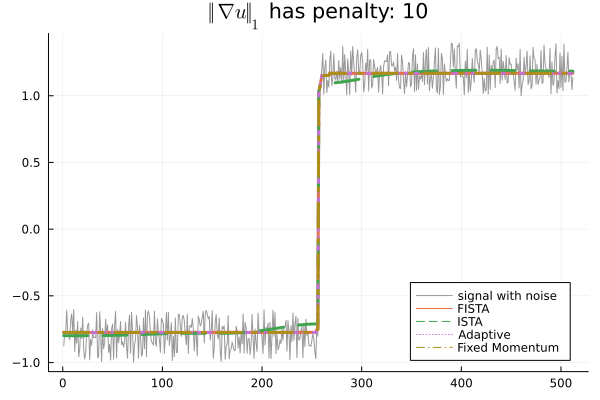
\includegraphics[width=10cm]{Assets/recovered_signal.png}    
        \end{figure}
        
    \end{frame}
    \begin{frame}{One Big Bummer}
        \begin{figure}
            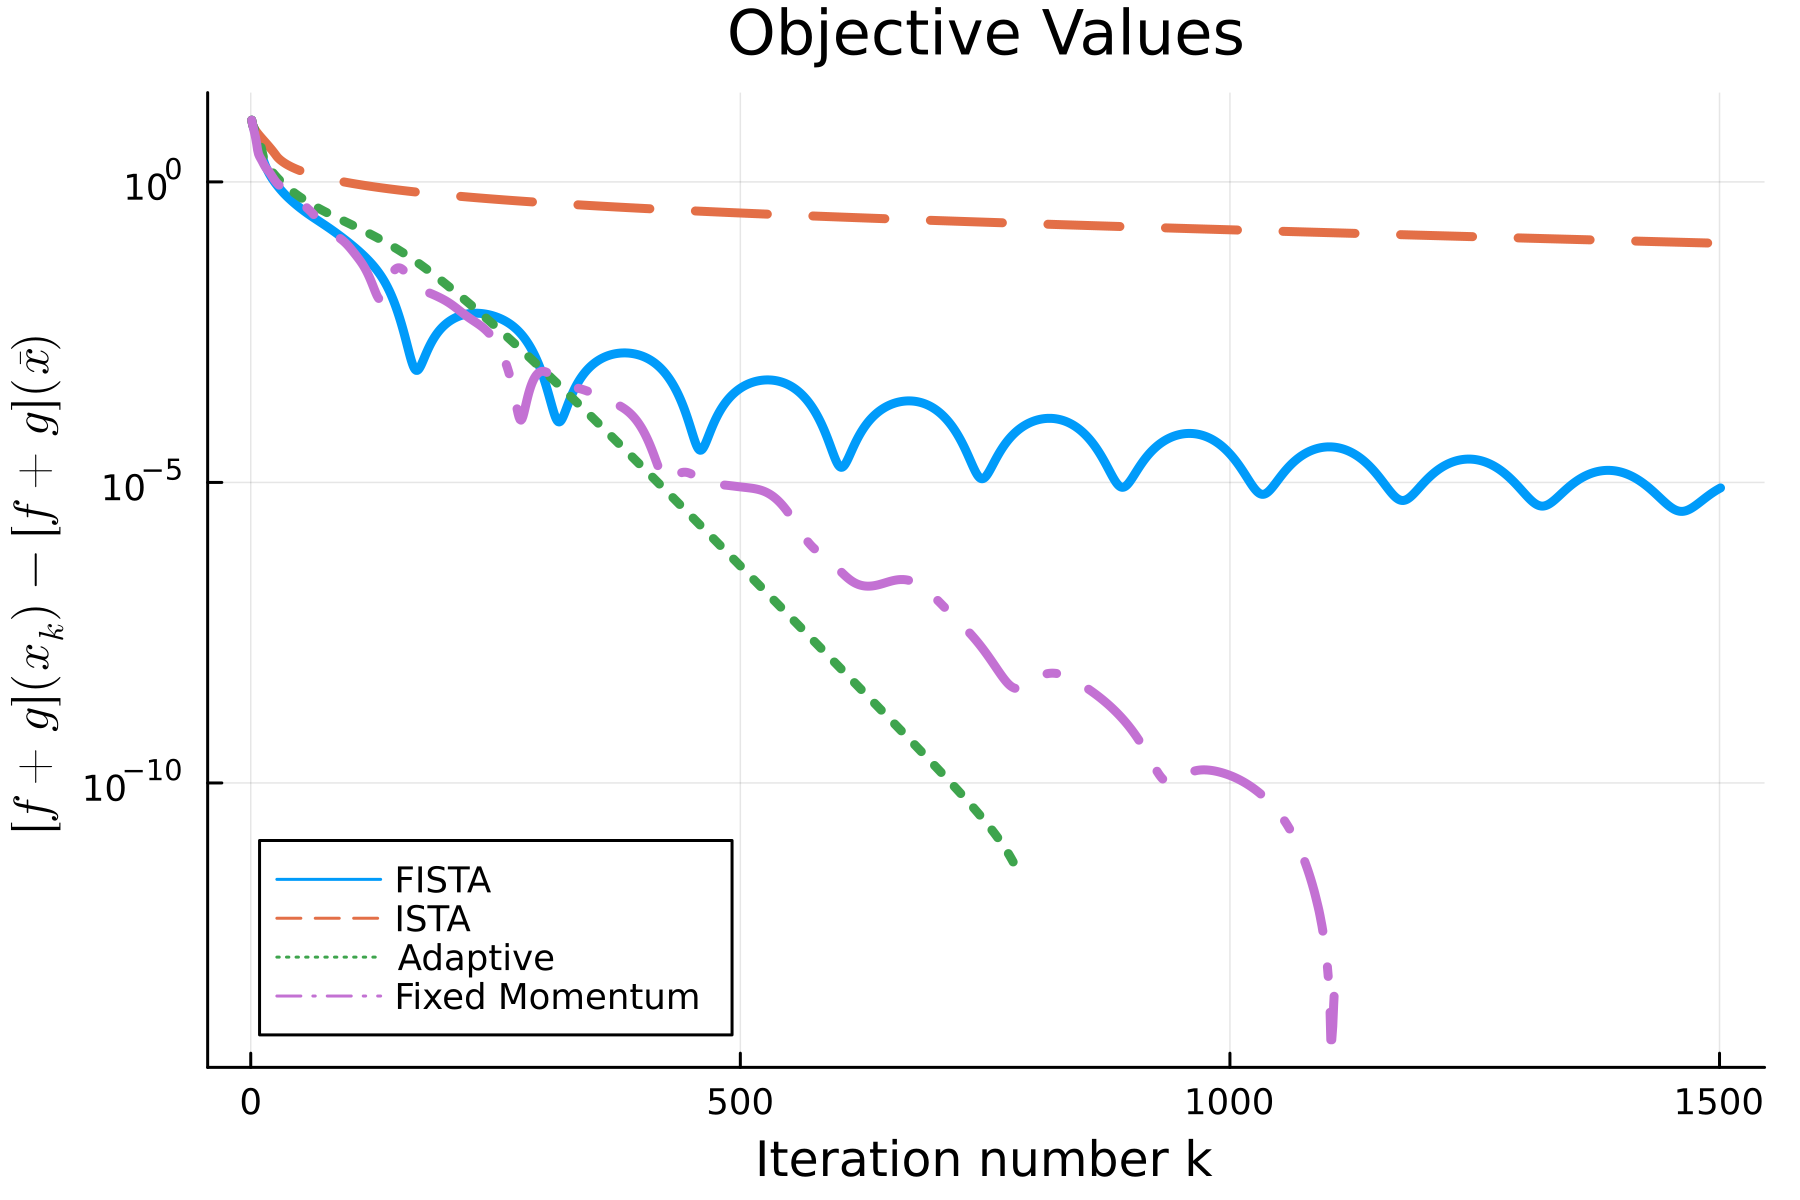
\includegraphics[width=10cm]{Assets/obj_vals.png}
        \end{figure}
    \end{frame}
    \begin{frame}{One Big Bummer}
        \begin{figure}
            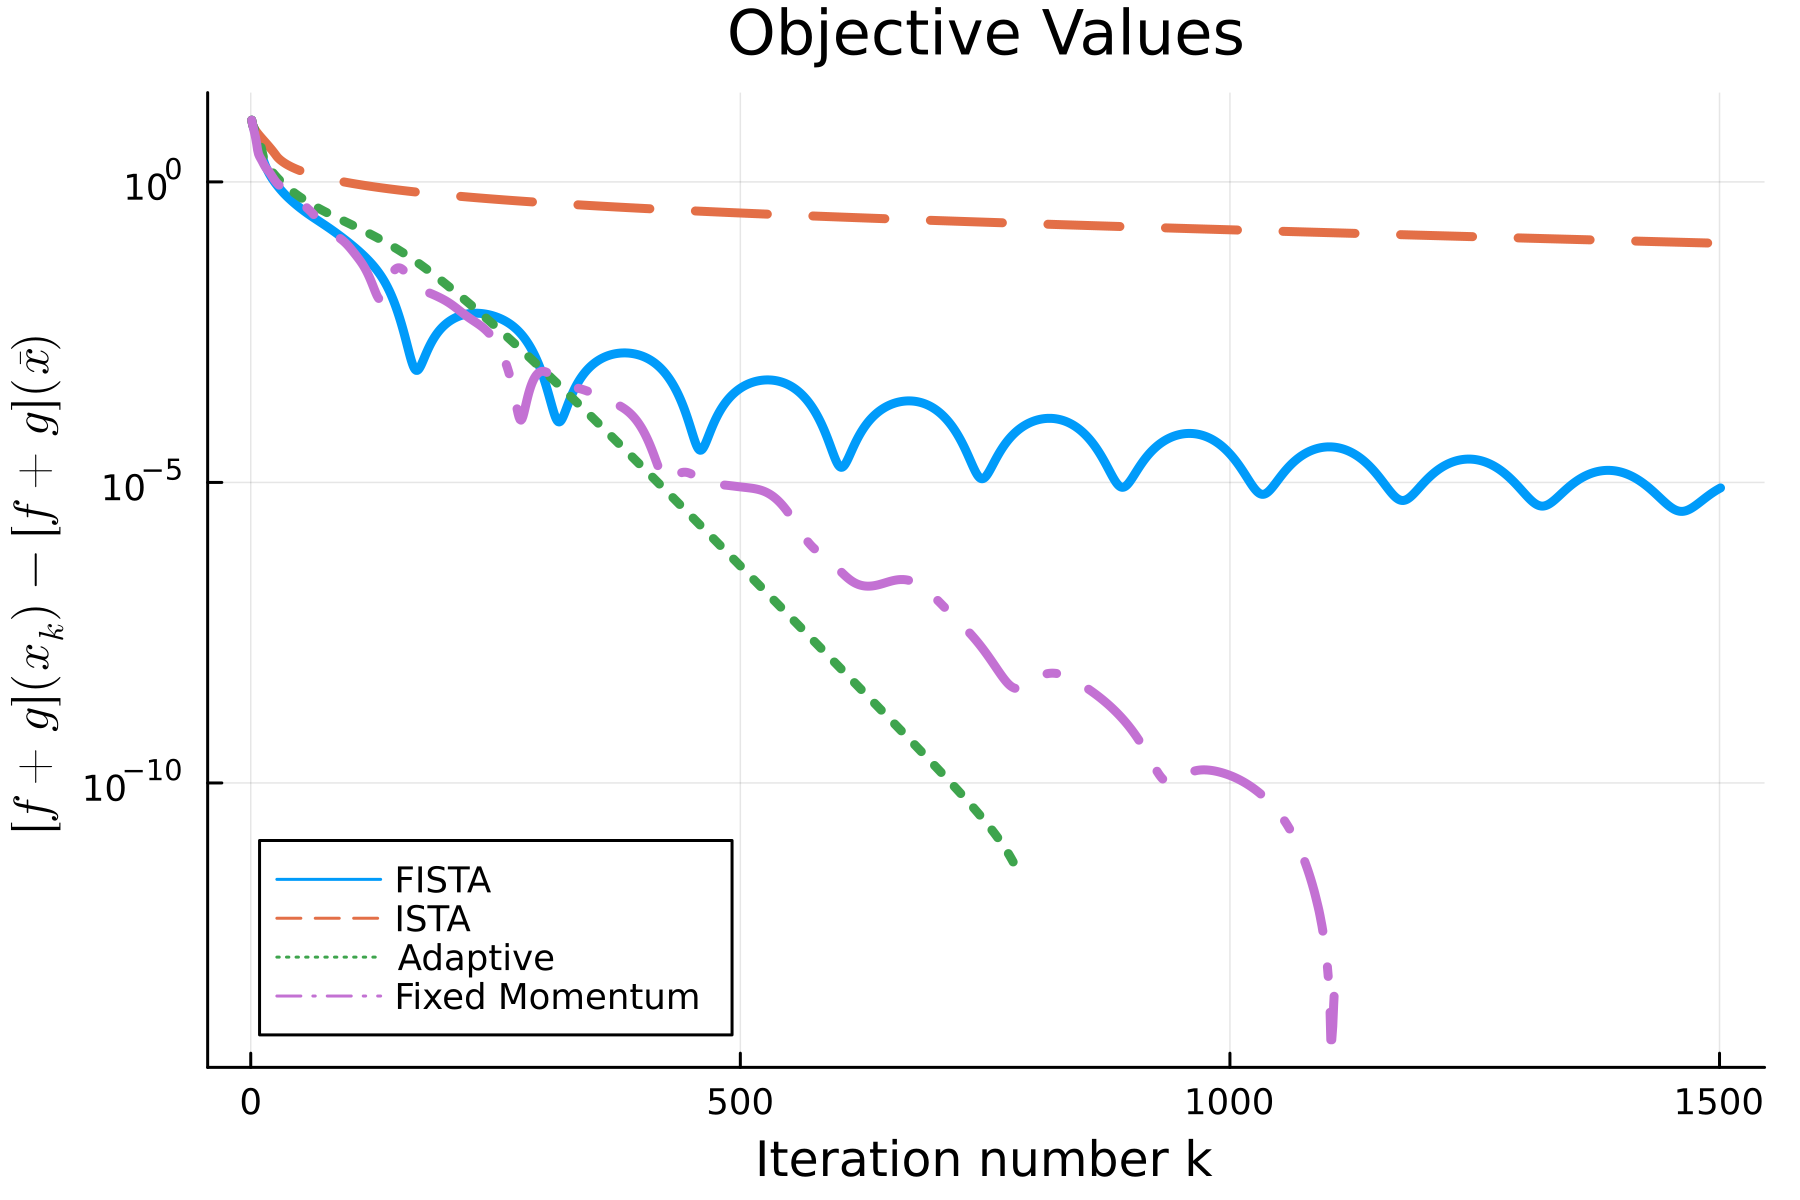
\includegraphics[width=6cm]{Assets/obj_vals.png}
        \end{figure}
        Main observations
        \begin{itemize}
            \item [1.] FISTA is non-robust to strong convexity; it experiences the same $\mathcal (1/k^2)$. 
            \item [2.] However, ISTA would be $\mathcal O(1 - 1/\kappa)^k)$ under strong convexity, with $\kappa = L/\sigma$, for $L$-Lipschitz smooth and $\sigma$ strongly on the smooth part of the FB splitting objective. 
        \end{itemize}
    \end{frame}
        
    
\section{Literature Review}
    \begin{frame}{Generic FISTA}
        We introduce the below algorithm \ref*{alg:generic_FISTA} to expedite presentation. 
        \begin{algorithm}[H]
            \begin{algorithmic}[1]
                \STATE{\textbf{Input: }($g, h, x^{(0)}$)}
                \STATE{$y^{(0)} = x^{(0)}$, $\kappa = L/\sigma$} 
                \FOR{$k = 0, 1, \cdots$}
                    \STATE{$x^{(k + 1)} = T_L y^{(k)}$}
                    \STATE{$y^{(k + 1)} = x^{(k + 1)} + \theta_{k + 1}(x^{(k + 1)} - x^{(k)})$}
                    \STATE{Execute subroutine $\mathcal S$. }
                \ENDFOR
            \end{algorithmic}
            \caption{Generic FISTA}
            \label{alg:generic_FISTA}
        \end{algorithm}
        Changing $T_L$, $\theta_{k + 1}$, and $\mathcal S$ yield different variants. 
    \end{frame}


\section{Nesterov Lower Bound}
    

\section{V-FISTA Under Strong Convexity}

\section{Numerical Results}
    
\section{References}
    \begin{frame}{References}
        
        \bibliography{refs.bib}
    \end{frame}

\end{document}